\documentclass{ctexart}

\usepackage[dvipsnames]{xcolor}
\usepackage{hyperref}
\usepackage{amsmath}
\usepackage{amsthm}
\usepackage{graphicx}
\usepackage{listings}
\usepackage{tcolorbox}
\usepackage{geometry}
\usepackage{amsmath}
\usepackage{longtable}
\usepackage{array}
\usepackage{titlesec}
\usepackage{fontspec}
\usepackage{xeCJK}
\usepackage{setspace}


\geometry{a4paper,margin=1in}

\hypersetup{colorlinks=true, pdfstartview=FitV, 
linkcolor=BrickRed,citecolor=BrickRed, urlcolor=BrickRed}

\lstset{
	basicstyle=\ttfamily,
	language=Python,
	xleftmargin=0pt,
	frame=none
}

\titleformat{\title}
{\bfseries\fontsize{24pt}{24pt}\selectfont} % 二号字体,黑体
{} % 空白的标签
{0pt} % 标题标签和标题正文之间的水平距离
{} % 标题的内容

% 设置英文字体为Arial
\setmainfont{Arial}

\titleformat{\section}
{\bfseries\fontsize{12pt}{14pt}\selectfont} % 小四号,黑体
{\thesection}{1em}{}

\titleformat{\subsection}
{\bfseries\fontsize{10.5pt}{14pt}\selectfont} % 五号,黑体
{\thesubsection}{1em}{}


% 设置段落格式
\usepackage{parskip}
\setlength{\parskip}{12pt} % 段前空12pt

\ctexset{
section = {
format = \raggedright\Large\bfseries,
}
}

\newcommand{\abstractnamefont}{\songti\fontsize{9pt}{14pt}\selectfont}
\renewcommand{\abstractname}{\abstractnamefont 摘要}

\title{基于python的全球人口数据分析与可视化}
\author{\fontsize{14pt}{14pt}
\selectfont 杨施诚,罗鹍,杨涛}
\date{\today}

\begin{document}
    \maketitle
    \begin{abstract}
        {\noindent 本文旨在利用Python进行全球人口数据的分析与可视化,以揭示全球及各国人口增长的趋势和特点。通过从Our World in Data网站下载的世界人口数据集,我们对数据进行了清洗和转换,并分析了全球和各国的总出生人数和总死亡人数、每年的出生和死亡动态、以及各国的出生率和死亡率。本文还包括多个可视化图表,以直观展示这些数据分析结果。研究结果显示,全球和各国的人口动态具有显著差异,这些差异反映了地理、经济和文化因素对人口变化的影响。通过深入的数据分析,我们识别出了影响人口增长的关键因素,并为政策制定和学术研究提供了数据支持。}
        \par\noindent \textbf{关键词:}全球人口、数据分析、数据可视化、出生率、死亡率、Python、Our World in Data
    \end{abstract}

    \newpage
    \tableofcontents

    \newpage
    \section{\textbf{引言}}
    	\subsection{\textbf{背景介绍}}
    •	全球人口增长是一个重要的社会经济现象,对资源分配、环境保护和经济发展有深远的影响。\par 
    •	随着全球人口的不断增长,出生率和死亡率的变化对人口结构和社会发展起到了关键作用\par 
    •	了解和分析这些数据可以帮助政策制定者和研究人员更好地理解人口动态,并制定有效的策略应对未来挑战。
    	\subsection{\textbf{研究目的}}
    •	本次数据分析的主要目的是利用Python进行全球人口数据的分析与可视化,以揭示全球及各国人口增长的趋势和特点。\par 
    •	具体任务包括数据获取与初步处理、数据分析总览、时间序列分析和统计分析。\par 
    •	通过数据可视化技术直观地展示全球和各国的人口变化趋势,为相关研究提供支持。
    	\subsection{\textbf{数据来源与方法概述}}
    •	本研究使用的数据集来源于Our World in Data网站,该数据集包含全球各国的出生和死亡数据。\par 
    •	使用Pandas进行数据读取与初步处理,Matplotlib进行数据可视化,NumPy进行统计分析\par 
    •	数据处理包括数据清洗、缺失值处理以及字符串处理技术清洗不规范字符或格式。
    	\subsection{\textbf{研究意义}}
    •	通过对全球和各国人口数据的详细分析与可视化,可以揭示出生率和死亡率的变化趋势,为人口研究提供数据支持。\par 
    •	分析结果有助于理解全球人口增长的现状和未来发展趋势,为政策制定和学术研究提供参考。
    \par \noindent
    这部分内容将帮助读者了解研究的背景、目的、数据来源和方法,以及研究的意义,从而为后续的章节提供清晰的导向。
    
    
    \section{\textbf{题目1:数据筛查}}
    
    \noindent 在数据筛查阶段,我们采取了系统化的方法来处理和整理全球人口相关的数据集。以下是具体的步骤和方法:

    \subsection{\textbf{数据下载与读取}}

    \noindent 首先,我们从Our World in Data网站下载了世界人口数据、出生人口数据和死亡人口数据的CSV格式数据集。使用os库进行准确的读取文件后,使用Python的Pandas模块读取这些数据集,以便进行进一步处理。

    \subsection{\textbf{初步数据检查}}  

    \noindent 在读取数据后,我们对数据进行了初步检查,确保数据的正确性和完整性。这包括查看前几行数据,确认数据是否正确读取,以及检查是否存在缺失值和重复行。

    \subsection{\textbf{数据清洗}}

    \noindent 为了确保数据的质量和一致性,我们采用了多种数据清洗方法:\par 

	\noindent •	数据筛选:从总人口数据中保留需要的列(国家名称、年份和人口总数),同样处理出生人口数据和死亡人口数据,以简化数据结构,提高分析效率。\par \noindent 
	•	处理缺失值:根据缺失值的分布和重要性,采取不同的处理策略。对随机分布的少量缺失值,直接删除;对重要且缺失值集中的特征,采用均值填充、中位数填充或基于回归模型的预测填充方法。\par \noindent 
	•	数据类型转换:检查并统一数据类型,确保所有数值类型一致,避免类型不匹配的错误。\par \noindent 
	•	数据一致性处理:对不同来源和格式的数据进行标准化处理,统一数值单位,并通过去重操作消除重复的数据记录。此外,使用正则表达式清洗数据中的不规范字符或格式,提高数据的质量。

    \subsection{\textbf{数据转换与输出}}

    \noindent 清洗后的数据被重新输出为新的CSV文件,以便后续的数据分析和模型构建。通过这种方式,我们确保了数据的可用性和高质量,为后续分析奠定了坚实的基础。

    \subsection{\textbf{总结}}

    \noindent 在数据筛查过程中,我们系统地进行了数据下载、初步检查和清洗,通过处理缺失值、无效数据、统一数据类型和标准化处理,显著提高了数据的质量和一致性。特别是使用正则表达式有效清洗了数据中的不规范字符或格式。最终,清洗后的数据输出为新的CSV文件,为后续的数据分析和模型构建提供了可靠的数据基础。
    \par \vspace{1cm} \noindent \emph{我们将写好的数据文件放置在one.py}
    \section{\textbf{题目2:数据分析详细过程及总结意见}}
    
    \noindent 在第二步的数据分析中,我们先使用os库正确读取并更改目录位置防止出错,通过使用Python的Pandas和NumPy库对全球和各国的人口数据进行了深入探索和分析。以下是我们的分析过程及相关意见:
    
    \subsection{\textbf{数据分析过程总结}}
    
    1. 全球总出生和死亡人数分析:
    我们首先计算了全球的总出生人数和总死亡人数,以获得对全球人口动态的整体了解。
    
    2. 各国总出生和死亡人数分析:
    通过对数据按国家分组并求和,我们得到了每个国家的总出生人数和总死亡人数,进一步分析了各国在人口增长和减少方面的贡献。
    
    3. 出生和死亡人数最多的国家:
    通过排名分析,我们识别出了出生人数和死亡人数最多的前十个国家,从而揭示了全球人口变化的重要驱动因素。
    
    4. 全球及选定国家每年人口动态分析:
    我们研究了全球每年出生和死亡人数的变化趋势,同时也深入分析了选定国家(如美国、印度、巴西)的人口动态变化情况,以捕捉长期趋势和突发变化。
    
    5. 全球和各国的出生率和死亡率分析:
    我们计算并比较了全球和各国的出生率和死亡率,这些指标为评估人口增长和健康状况提供了重要数据支持。
    
    6. 选定国家的基本统计数据分析:
    最后,我们分析了选定国家的基本统计数据,包括出生人数和死亡人数的均值、中位数和方差,以深入了解其人口变化的稳定性和波动性。
    
    \subsection{\textbf{总结与意见}}
    
    \noindent 在本次数据分析过程中,我们深入挖掘了人口数据背后的故事和趋势,发现了一些关键的发现和趋势:\par 
    
    \noindent 人口增长的驱动因素:通过分析出生和死亡人数,我们可以识别出影响全球和各国人口增长的关键因素,例如经济发展、医疗进步和社会政策变化等。\par 
    
    \noindent 地区和国家间的差异:不同国家和地区在人口动态方面存在显著差异,这些差异反映了地理、经济和文化因素对人口变化的影响。\par 
    
    \noindent 长期趋势和突发变化:通过年度数据分析,我们可以捕捉到长期的人口变化趋势,同时也能够识别出可能导致人口变动的突发事件和趋势变化。\par 
    
    \noindent 综上所述,通过这些分析,我们不仅加深了对全球和各国人口动态的理解,还为未来制定更有效的人口政策和社会发展战略提供了数据支持。在进行类似的数据分析时,持续关注数据质量和准确性,并结合深入的领域知识和背景信息,将有助于更准确地理解和解释人口数据背后的复杂变化。
    \par \noindent 使用'w+'和'a'方法规定一个文档,并将上述所有输出依次输出到'output'文件中.
    \par \noindent \emph{我们将写好的文件放在two.py中,更改后是two\_ 1.py}
    
    \section{\textbf{题目3:可视化}}
    \noindent 本部分主要使用pandas库对文件\textbf{birth.csv,birth\_rt.csv,death.csv,death\_rt.csv}文件进行可视化操作,同样在开始使用os库更改目录位置
    \par \noindent 定义了color函数以随机颜色,并书写目录位置将所有文件保存至'output'文件中.
    
    \subsection{\textbf{出生死亡人数图表绘制}}
    \noindent 简要观察图表,发现第一小问只需考虑world的数据即18072-18143的位置,使用该位置数据绘制出生人数表格,并同理运用至死亡人数
    \subsection{\textbf{前十个出生人数和死亡人数最多的国家图表绘制}}
    \noindent 使用简单的sorted函数排序十个国家并类似地使用第一小问的绘制方法构造柱状图,但是发现会出现例如'world','undeveloped reigons'这样不符合
    题干要求的内容如下
    \begin{figure}[h!]
        \centering
        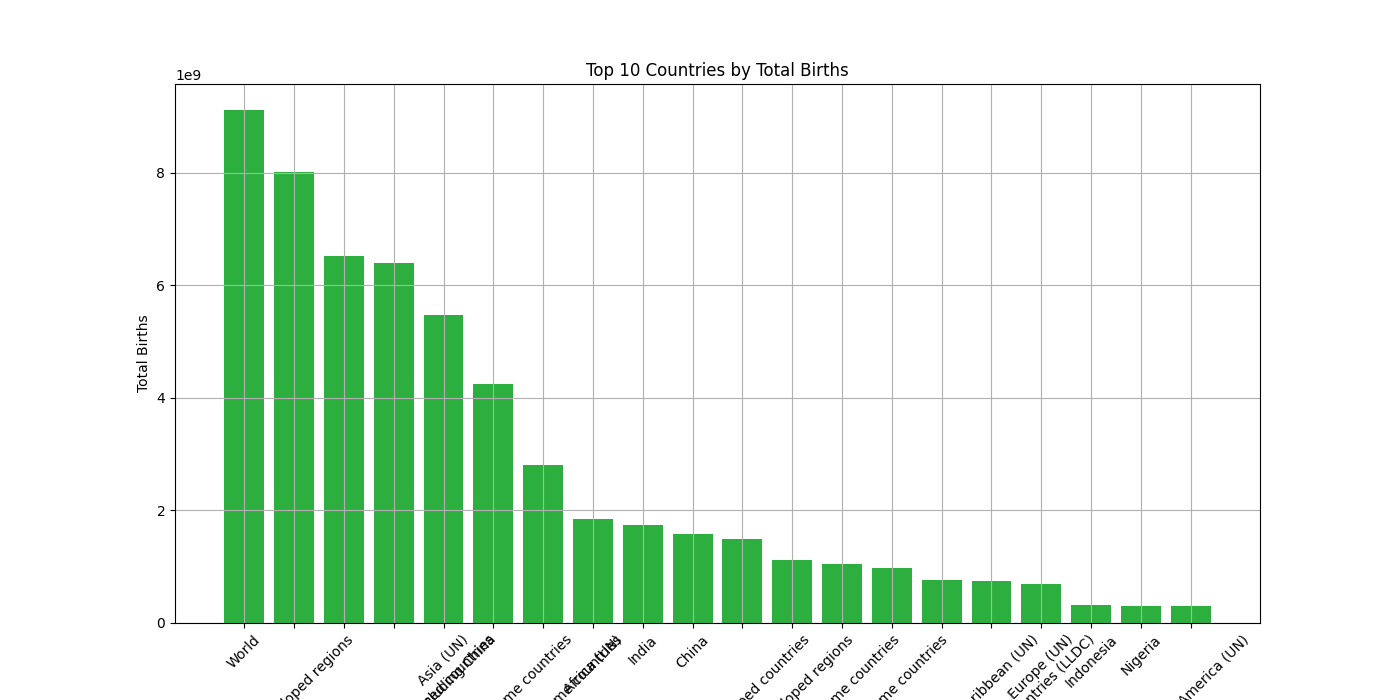
\includegraphics[width=0.5\textwidth]{img/world_most_10_birth_in_year.png}
        \caption{出生人数前十}
        \label{1}
    \end{figure}

    \begin{figure}[h!]
        \centering
        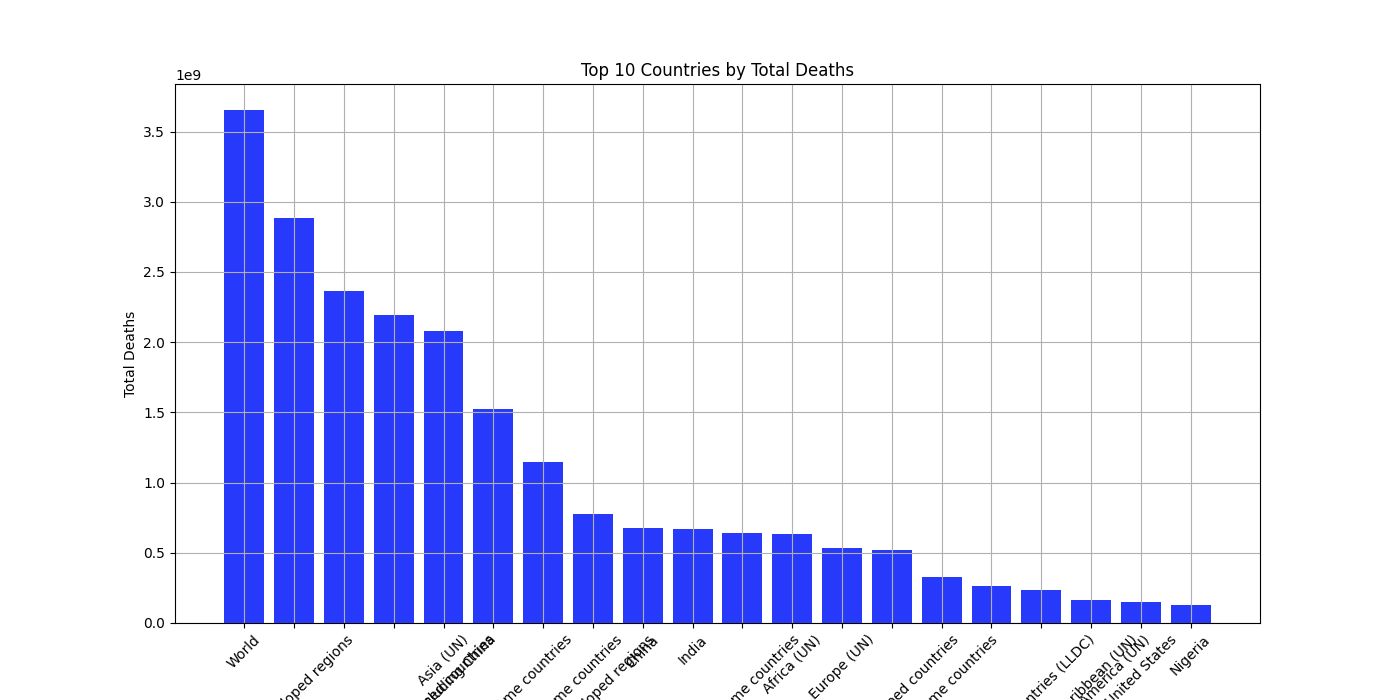
\includegraphics[width=0.5\textwidth]{img/world_most_10_death_in_year.png}
        \caption{死亡人数前十}
        \label{2}
    \end{figure}
    
    \noindent 因此我们遍历了整个第二维的列行标签,选出不是国家的名称的集合,并在绘图中选择不含这些名称的前十名
    \begin{figure}[h!]
        \centering
        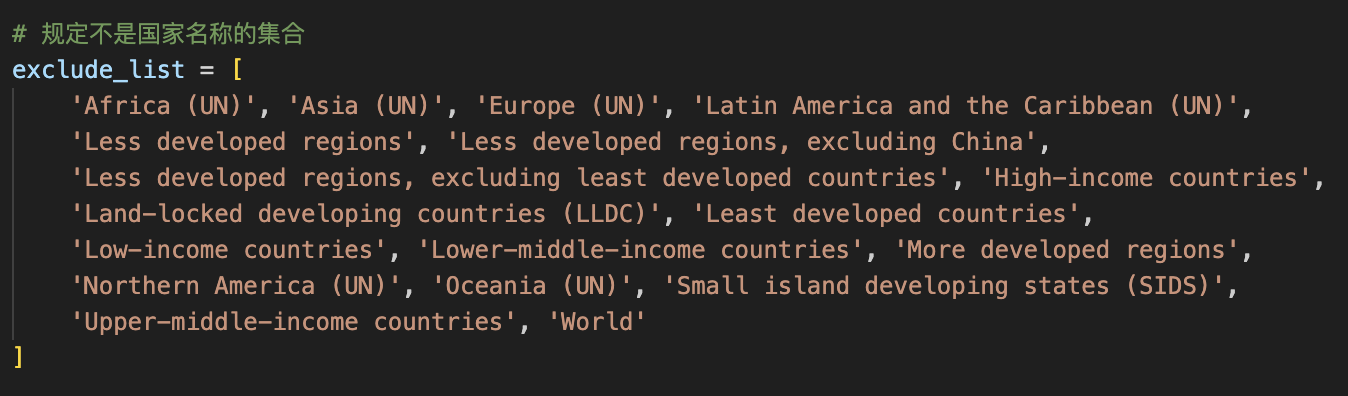
\includegraphics[width=0.5\textwidth]{img/excluded.png}
        \caption{不是国家的名称合集}
        \label{3}
    \end{figure}
    \noindent 然后此时绘图就没有出现任何错误,并且符合我们的预期:中国和印度人口很多.
    \subsection{\textbf{全球每年新增出生人数和新增死亡人数的折线图绘制}}
    \noindent 分析本题目,发现需要对人数做差,因此主要使用了以下
    \begin{lstlisting}[language=Python]
        kk=2;[mdd,ndd]=size(dd);
        br_yr = df_b.groupby('Year')['Births'].sum().reset_index()
        br_yr['Birth Increase'] = br_yr['Births'].diff().fillna(0)
        dt_yr = df_d.groupby('Year')['Deaths'].sum().reset_index()
        dt_yr['Death Increase'] = dt_yr['Deaths'].diff().fillna(0)
    \end{lstlisting}
    的代码做差,根据matplot对时间做了折线图,下面一提同理,但需要使用,挑选出几个国家,此处挑选美国,印度和中国.

    \subsection{\textbf{不同国家出生率和死亡率的对比图绘制}}
    \noindent 最后一题是选取两个国家分析他们的出生和死亡率,因此挑选rate.csv文件,
    以下是代码设计:
    \begin{lstlisting}[language=Python]
        kk=2;[mdd,ndd]=size(dd);
        def b_d_compare(country1, country2):
    birth_color1 = color()
    death_color1 = color()
    birth_color2 = color()
    death_color2 = color()

    # 过滤出选定国家的出生率和死亡率数据
    df_br1 = df_br[df_br['Country name'] == country1].copy()
    df_dr1 = df_dr[df_dr['Country name'] == country1].copy()
    df_br2 = df_br[df_br['Country name'] == country2].copy()
    df_dr2 = df_dr[df_dr['Country name'] == country2].copy()

    plt.figure(figsize=(14, 7))

    # 绘制国家1的出生率和死亡率折线图
    plt.plot(df_br1['Year'], df_br1['Birth rate'], color=
    birth_color1, marker='o', linestyle='-', label=f'{country1} Birth Rate')
    plt.plot(df_dr1['Year'], df_dr1['Death rate'], color=
    death_color1, marker='x', linestyle='--', label=f'{country1} Death Rate')

    # 绘制国家2的出生率和死亡率折线图
    plt.plot(df_br2['Year'], df_br2['Birth rate'], color=
    birth_color2, marker='o', linestyle='-', label=f'{country2} Birth Rate')
    plt.plot(df_dr2['Year'], df_dr2['Death rate'], color=
    death_color2, marker='x', linestyle='--', label=f'{country2} Death Rate')

    plt.xlabel('Year')
    plt.ylabel('Rate')
    plt.title(f'Birth and Death Rate Comparison: {country1} vs {country2}')
    plt.legend()
    plt.grid(True)

    # 输出
    output_path = os.path.join(output_dir, f'{country1}_{country2}比较.png')
    plt.savefig(output_path)
    plt.close()
        
    \end{lstlisting}
    \par \vspace{1cm} \noindent \emph{我们将写好的数据文件放置在three.py}

    \section{\textbf{总括操作}}
    \noindent 考虑到我们将代码全部定义成了功能块,因此在main中引用,很快就可以得出结果,并输出在'output'文件夹中
    如下所示:
        \begin{lstlisting}[language=Python] %设置不同语言即可。
        kk=2;[mdd,ndd]=size(dd);
        import os
        import one as o
        import two_1 as tw
        import three as tr

        print("hello world!")

        \end{lstlisting}
    这之后调用函数就可以实现全部功能并生成在'output'文件夹中,整个文件放置在\href{https://github.com/LucyJesus/Py_DataAny_project.git}{GitHub}中



    \newpage
    \appendix
    \section{附录一:主代码(全部操作的整合)}
        \begin{lstlisting}[language=Python] %设置不同语言即可。
        kk=2;[mdd,ndd]=size(dd);
        import os
        import one as o
        import two_1 as tw
        import three as tr


        print("hello world!")
        script_dir = os.path.dirname(os.path.abspath(__file__))
        os.chdir(script_dir)
        ################################################


        #主代码部分
        o.clean()

        tw.global_all()
        tw.most_10b()
        tw.most_10d()
        tw.in_year_global_b_d()
        tw.global_b_d_r()
        tw.each_b_d_r()
        tw.combine()

        tr.birth_and_death_tt()
        tr.most_10_birth()
        tr.most_10_death()
        tr.yearly_birth_and_death_increase_plot()
        tr.daily_increase_plot()
        tr.b_d_compare('United States', 'China')


        \end{lstlisting}
    \newpage
    \section{附录二:one.py(题目1的整合)}
    \tiny
        \begin{lstlisting}[language=Python] %设置不同语言即可。
            kk=2;[mdd,ndd]=size(dd);
            import pandas as pd
            import os

            # 打印当前工作目录
            # print(os.getcwd())

            # 确保文件路径正确
            def clean():
                population_path = "data/population-and-demography.csv"
                birth_path = "data/population-and-demography (1).csv"
                death_path = "data/population-and-demography (2).csv"
                output_folder = "output"
                if not os.path.exists(output_folder):
                    os.makedirs(output_folder)
                # 读取文件
                population = pd.read_csv(population_path)  # 读取总人口数数据
                birth = pd.read_csv(birth_path)   # 读取出生人口数据
                death = pd.read_csv(death_path)   # 读取死亡人口数据
                #下面进行数据清洗和整理无效数据
                data1 = population.loc[:,'Country name':'Population']    #去年龄段 保留总人口数
                list1= data1['Country name'].tolist()
                list2=data1['Year'].tolist()
                list3= data1['Population'].tolist()
                s= {'Year':list2,'Population':list3}
                data_Population = pd.DataFrame(s,[list1])              #转换国家或地区为行标签

                data2 = birth.loc[:,'Country name':'Births']    #同理 出生人数
                list1= data2['Country name'].tolist()
                list2=data2['Year'].tolist()
                list3= data2['Births'].tolist()
                s= {'Year':list2,'Births':list3}
                data_Birth = pd.DataFrame(s,[list1]) 

                data3 = death.loc[:,'Country name':'Deaths']  #死亡人数
                list1= data3['Country name'].tolist()
                list2=data3['Year'].tolist()
                list3= data3['Deaths'].tolist()
                s= {'Year':list2,'Deaths':list3}
                data_Death = pd.DataFrame(s,[list1]) 


                data_Birth['Births']=data_Birth['Births'].astype('int64')   #修改数据类型为整形

                population_output_path = os.path.join(output_folder, '人口数据(已清洗).csv')
                birth_output_path = os.path.join(output_folder, '出生数据(已清洗).csv')
                death_output_path = os.path.join(output_folder, '死亡数据(已清洗).csv')

                # 输出为csv文件
                data_Population.to_csv(population_output_path, index=False)
                data_Birth.to_csv(birth_output_path, index=False)
                data_Death.to_csv(death_output_path, index=False)
                
        \end{lstlisting}
    \newpage

    \section{附录三:$two_1$.py(题目2的整合)}
    \tiny
        \begin{lstlisting}[language=Python] %设置不同语言即可。
            kk=2;[mdd,ndd]=size(dd);
            import pandas as pd
            import os

            # 读取CSV文件
            deaths_df = pd.read_csv(r'data/birth.csv')
            births_df = pd.read_csv(r'data/death.csv')
            population_df = pd.read_csv(r'data/population.csv')

            # 合并数据帧
            df = pd.merge(births_df, deaths_df, on=['Country name', 'Year'], how='inner')
            df = pd.merge(df, population_df, on=['Country name', 'Year'], how='inner')

            # 去除列名中的空格
            df.columns = df.columns.str.strip()

            # 检查缺失值并填充
            df.fillna(0, inplace=True)

            # 确认数据类型并转换
            df['Births'] = df['Births'].astype(int)
            df['Deaths'] = df['Deaths'].astype(int)
            df['Population'] = df['Population'].astype(int)

            # 总出生死亡人数
            global_births = df['Births'].sum()
            global_deaths = df['Deaths'].sum()

            # 创建输出目录
            script_dir = os.path.dirname(os.path.abspath(__file__))
            output_dir = os.path.join(script_dir, 'output')
            if not os.path.exists(output_dir):
                os.makedirs(output_dir)

            output_path = os.path.join(output_dir, '第二题输出文件.txt')

            def global_all():
                with open(output_path, 'w+') as f:
                    f.write(f"全球总出生: {global_births}\n")
                    f.write(f"总死亡: {global_deaths}\n")

            # 按国家计算总出生人数和总死亡人数
            country_totals = df.groupby('Country name')[['Births', 'Deaths', 'Population']].sum()

            # 过滤掉非国家实体
            exclude_list = [
                'Africa (UN)', 'Asia (UN)', 'Europe (UN)', 'Latin America and the Caribbean (UN)', 
                'Less developed regions', 'Less developed regions, excluding China', 
                'Less developed regions, excluding least developed countries', 'High-income countries', 
                'Land-locked developing countries (LLDC)', 'Least developed countries', 
                'Low-income countries', 'Lower-middle-income countries', 'More developed regions', 
                'Northern America (UN)', 'Oceania (UN)', 'Small island developing states (SIDS)', 
                'Upper-middle-income countries', 'World'
            ]

            country_totals = country_totals[~country_totals.index.isin(exclude_list)]

            # 找出出生人数最多的前十个国家
            def most_10b():
                top10_births = country_totals['Births'].nlargest(10)
                with open(output_path, 'a') as f:
                    f.write("出生人数最多的前十个国家:\n")
                    f.write(f"{top10_births}\n")

            # 找出死亡人数最多的前十个国家
            def most_10d():
                top10_deaths = country_totals['Deaths'].nlargest(10)
                with open(output_path, 'a') as f:
                    f.write("死亡人数最多的前十个国家:\n")
                    f.write(f"{top10_deaths}\n")

            # 按年份计算全球每年出生人数和死亡人数
            def in_year_global_b_d():
                annual_global_totals = df.groupby('Year')[['Births', 'Deaths']].sum()
                with open(output_path, 'a') as f:
                    f.write("按年份计算全球每年出生人数和死亡人数:\n")
                    f.write(f"{annual_global_totals}\n")

            # 选择要分析的国家
            selected_countries = ['United States', 'India', 'Brazil']
            annual_country_totals = df[df['Country name'].isin(selected_countries)].groupby(['Year', 'Country name'])[['Births', 'Deaths']].sum().reset_index()

            # 计算全球出生率和死亡率
            def global_b_d_r():
                global_birth_rate = global_births / df['Population'].sum() * 1000
                global_death_rate = global_deaths / df['Population'].sum() * 1000
                with open(output_path, 'a') as f:
                    f.write(f"Global birth rate: {global_birth_rate:.2f} per 1000 people\n")
                    f.write(f"Global death rate: {global_death_rate:.2f} per 1000 people\n")

            # 计算各国出生率和死亡率
            def each_b_d_r():
                country_totals['birth_rate'] = country_totals['Births'] / country_totals['Population'] * 1000
                country_totals['death_rate'] = country_totals['Deaths'] / country_totals['Population'] * 1000
                with open(output_path, 'a') as f:
                    f.write("各国出生率和死亡率:\n")
                    f.write(f"{country_totals[['birth_rate', 'death_rate']]}\n")

            # 计算选定国家的基本统计数据
            def combine():
                selected_country_stats = df[df['Country name'].isin(selected_countries)]
                country_stats = selected_country_stats.groupby('Country name')[['Births', 'Deaths']].agg(['mean', 'median', 'var'])
                with open(output_path, 'a') as f:
                    f.write("选定国家的基本统计数据:\n")
                    f.write(f"{country_stats}\n")


        \end{lstlisting}
    \newpage

    \section{附录四:three.py(题目3的整合)}
    \tiny
        \begin{lstlisting}[language=Python] %设置不同语言即可。
            kk=2;[mdd,ndd]=size(dd);
            import pandas as pd
            import numpy as np
            import csv
            import os
            import matplotlib.pyplot as plt
            import random


            #print("hello world!")

            # 获取脚本所在目录
            script_dir = os.path.dirname(os.path.abspath(__file__))
            # print("Script directory:", script_dir)

            # 切换工作目录到脚本所在目录
            os.chdir(script_dir)

            # 规定不是国家名称的集合
            exclude_list = [
                'Africa (UN)', 'Asia (UN)', 'Europe (UN)', 'Latin America and the Caribbean (UN)', 
                'Less developed regions', 'Less developed regions, excluding China', 
                'Less developed regions, excluding least developed countries', 'High-income countries', 
                'Land-locked developing countries (LLDC)', 'Least developed countries', 
                'Low-income countries', 'Lower-middle-income countries', 'More developed regions', 
                'Northern America (UN)', 'Oceania (UN)', 'Small island developing states (SIDS)', 
                'Upper-middle-income countries', 'World'
            ]


            output_dir = os.path.join(script_dir, 'output')
            if not os.path.exists(output_dir):
                    os.makedirs(output_dir)

            def color():
                a = random.random()
                b = random.random()
                c = random.random()
                return(a, b, c)

            # 读取 CSV 文件
            birth = os.path.join(script_dir, 'data', 'birth.csv')
            death = os.path.join(script_dir, 'data', 'death.csv')
            bir_rt = os.path.join(script_dir, 'data', 'birth_rate.csv')
            dea_rt = os.path.join(script_dir, 'data', 'death_rate.csv')

            df_b = pd.read_csv(birth)
            df_br = pd.read_csv(bir_rt)
            df_d = pd.read_csv(death)
            df_dr = pd.read_csv(dea_rt)

            def birth_and_death_tt():
                birth_color = color()
                death_color = color()
                df_b1 = df_b.loc[18072:18143, 'Year':'Births']
                df_d1 = df_d.loc[18072:18143, 'Year':'Deaths']
                plt.figure(figsize=(14, 7))

                plt.bar(df_b1['Year'] - 0.2, df_b1['Births'], width=0.4, color=birth_color, align='center', label='Births')
                plt.bar(df_d1['Year'] + 0.2, df_d1['Deaths'], width=0.4, color=death_color, align='center', label='Deaths')

                plt.xlabel('Year')  # 设置标题和标签
                plt.ylabel('Number')
                plt.title('World Total Births and Deaths in Year')
                plt.xticks(rotation=45)
                plt.legend()
                plt.grid(True)

                # 输出
                output_path = os.path.join(output_dir, '全球总出生和死亡人数的柱状图.png')
                plt.savefig(output_path)
                plt.close()


            def filter_countries(df):
                return df[~df['Country name'].isin(exclude_list)]

            def most_10_birth():
                # 过滤不是国家名称的条目
                flt_df = filter_countries(df_b)
                
                # 计算每个国家的总出生人数
                tt_b = flt_df.groupby('Country name')['Births'].sum().reset_index()
                tt_b = tt_b.sort_values(by='Births', ascending=False).head(10)

                # 绘制前十个出生人数最多的国家的柱状图
                plt.figure(figsize=(14, 7))
                plt.bar(tt_b['Country name'], tt_b['Births'], color=color())
                plt.xlabel('Country')
                plt.ylabel('Total Births')
                plt.title('Top 10 Countries by Total Births')
                plt.xticks(rotation=45)
                plt.grid(True)
                output_path = os.path.join(output_dir, '前十个出生人数最多的国家的柱状图.png')
                plt.savefig(output_path)


            def most_10_death():
                # 过滤不是国家名称的条目
                flt_df = filter_countries(df_d)
                tt_d = flt_df.groupby('Country name')['Deaths'].sum().reset_index()
                tt_d = tt_d.sort_values(by='Deaths', ascending=False).head(10)

                # 绘制前十个死亡人数最多的国家的柱状图
                plt.figure(figsize=(14, 7))
                plt.bar(tt_d['Country name'], tt_d['Deaths'], color=color())
                plt.xlabel('Country')
                plt.ylabel('Total Deaths')
                plt.title('Top 10 Countries by Total Deaths')
                plt.xticks(rotation=45)
                plt.grid(True)
                output_path = os.path.join(output_dir, '前十个死亡人数最多的国家的柱状图.png')
                plt.savefig(output_path)


            def yearly_birth_and_death_increase_plot():
                birth_color = color()
                death_color = color()
                br_yr = df_b.groupby('Year')['Births'].sum().reset_index()
                br_yr['Birth Increase'] = br_yr['Births'].diff().fillna(0)
                dt_yr = df_d.groupby('Year')['Deaths'].sum().reset_index()
                dt_yr['Death Increase'] = dt_yr['Deaths'].diff().fillna(0)

                # 绘制每年的新增出生和死亡人数折线图
                plt.figure(figsize=(14, 7))
                plt.plot(br_yr['Year'], br_yr['Birth Increase'], color=birth_color, marker='o', label='Birth Increase')
                plt.plot(dt_yr['Year'], dt_yr['Death Increase'], color=death_color, marker='x', label='Death Increase')
                plt.xlabel('Year')
                plt.ylabel('Annual Increase')
                plt.title('Global Annual Birth and Death Increase')
                plt.legend()
                plt.grid(True)

                # 输出
                output_path = os.path.join(output_dir, '全球每年新增出生和死亡人数的折线图.png')
                plt.savefig(output_path)
                plt.close()

            selected_countries = ['United States', 'India', 'China']

            def daily_increase_plot():
                for country in selected_countries:
                    # 过滤出该国家的出生和死亡数据
                    country_births = df_b[df_b['Country name'] == country].copy()
                    country_deaths = df_d[df_d['Country name'] == country].copy()
                    country_births['Birth Increase'] = country_births['Births'].diff().fillna(0)
                    country_deaths['Death Increase'] = country_deaths['Deaths'].diff().fillna(0)

                    # 绘制出生人数折线图
                    plt.figure(figsize=(14, 7))
                    plt.plot(country_births['Year'], country_births['Birth Increase'], color=color(), marker='o', label='Daily Birth Increase')
                    plt.plot(country_deaths['Year'], country_deaths['Death Increase'], color=color(), marker='x', label='Daily Death Increase')
                    plt.xlabel('Year')
                    plt.ylabel('Increase')
                    plt.title(f'Daily Birth and Death Increase in {country}')
                    plt.legend()
                    plt.grid(True)

                    # 保存文件到output目录
                    output_path = os.path.join(output_dir, f'{country}出生死亡人数折线图.png')
                    plt.savefig(output_path)
                    plt.close()


            def b_d_compare(country1, country2):
                birth_color1 = color()
                death_color1 = color()
                birth_color2 = color()
                death_color2 = color()

                # 过滤出选定国家的出生率和死亡率数据
                df_br1 = df_br[df_br['Country name'] == country1].copy()
                df_dr1 = df_dr[df_dr['Country name'] == country1].copy()
                df_br2 = df_br[df_br['Country name'] == country2].copy()
                df_dr2 = df_dr[df_dr['Country name'] == country2].copy()

                plt.figure(figsize=(14, 7))

                # 绘制国家1的出生率和死亡率折线图
                plt.plot(df_br1['Year'], df_br1['Birth rate'], color=birth_color1, marker='o', linestyle='-', label=f'{country1} Birth Rate')
                plt.plot(df_dr1['Year'], df_dr1['Death rate'], color=death_color1, marker='x', linestyle='--', label=f'{country1} Death Rate')

                # 绘制国家2的出生率和死亡率折线图
                plt.plot(df_br2['Year'], df_br2['Birth rate'], color=birth_color2, marker='o', linestyle='-', label=f'{country2} Birth Rate')
                plt.plot(df_dr2['Year'], df_dr2['Death rate'], color=death_color2, marker='x', linestyle='--', label=f'{country2} Death Rate')

                plt.xlabel('Year')
                plt.ylabel('Rate')
                plt.title(f'Birth and Death Rate Comparison: {country1} vs {country2}')
                plt.legend()
                plt.grid(True)

                # 输出
                output_path = os.path.join(output_dir, f'{country1}_{country2}比较.png')
                plt.savefig(output_path)
                plt.close()
    
        \end{lstlisting}
    \newpage

    \section{附录五:第二题输出文件}

    \tiny
    全球总出生: 60796835074 \par
    总死亡: 23635110902 \par
    
    出生人数最多的前十个国家: \par
    \begin{tabbing}
    \hspace{2cm} \= \kill
    \textbf{Country name} \> \textbf{Births} \\
    India \> 1736563802 \\
    China \> 1582454917 \\
    Indonesia \> 324234348 \\
    Nigeria \> 303496381 \\
    Pakistan \> 299225942 \\
    United States \> 272147302 \\
    Brazil \> 241549750 \\
    Bangladesh \> 231445437 \\
    Ethiopia \> 157685662 \\
    Mexico \> 154880593 \\
    \end{tabbing}
    
    死亡人数最多的前十个国家: \par
    \begin{tabbing}
    \hspace{2cm} \= \kill
    \textbf{Country name} \> \textbf{Deaths} \\
    China \> 678780442 \\
    India \> 666302479 \\
    United States \> 151933146 \\
    Nigeria \> 125277310 \\
    Indonesia \> 118821384 \\
    Russia \> 114779414 \\
    Pakistan \> 85006345 \\
    Bangladesh \> 80320627 \\
    Brazil \> 80309157 \\
    Japan \> 67949514 \\
    \end{tabbing}
    
    按年份计算全球每年出生人数和死亡人数: \par
    \begin{longtable}{|c|c|c|}
    \hline
    Year & Births & Deaths \\
    \hline
    1950 & 590102115 & 313586143 \\
    1951 & 595820717 & 311725766 \\
    1952 & 626077009 & 306455768 \\
    1953 & 627337344 & 305656586 \\
    1954 & 645605058 & 302785210 \\
    ... & ... & ... \\
    2017 & 970249655 & 367044003 \\
    2018 & 953204296 & 369702277 \\
    2019 & 943660177 & 373774673 \\
    2020 & 926922904 & 407332502 \\
    2021 & 920406730 & 448549176 \\
    \hline
    \end{longtable}
    
    Global birth rate: 26.29 per 1000 people \par
    Global death rate: 10.22 per 1000 people \par
    
    各国出生率和死亡率: \par
    \begin{longtable}{|c|c|c|}
    \hline
    Country name & birth\_rate & death\_rate \\
    \hline
    Afghanistan & 45.452162 & 15.710269 \\
    Albania & 23.388681 & 8.364540 \\
    Algeria & 30.881262 & 9.115526 \\
    American Samoa & 30.837994 & 5.321515 \\
    Andorra & 12.042302 & 5.840749 \\
    ... & ... & ... \\
    Wallis and Futuna & 28.031877 & 9.160690 \\
    Western Sahara & 26.945422 & 9.382617 \\
    Yemen & 42.352271 & 11.789009 \\
    Zambia & 43.716026 & 12.474797 \\
    Zimbabwe & 38.211001 & 12.104307 \\
    \hline

    \end{longtable}
    
    选定国家的基本统计数据: \par
    Country name ...
    \newpage

    \section{附录六:可视化图片}
    \begin{figure}[h!]
        \centering
        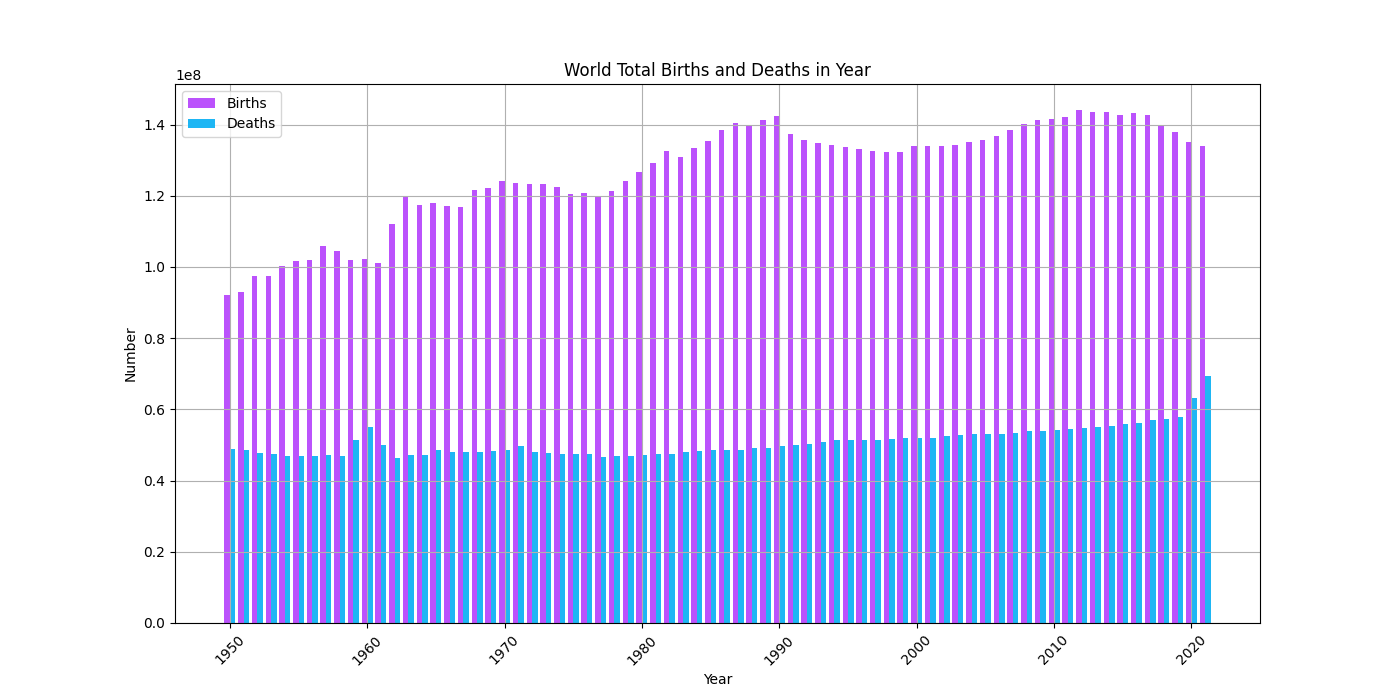
\includegraphics[width=0.5\textwidth]{img/全球总出生和死亡人数的柱状图.png}
        \caption{全球总出生和死亡人数的柱状图}
        \label{4}
    \end{figure}

    \begin{figure}[h!]
        \centering
        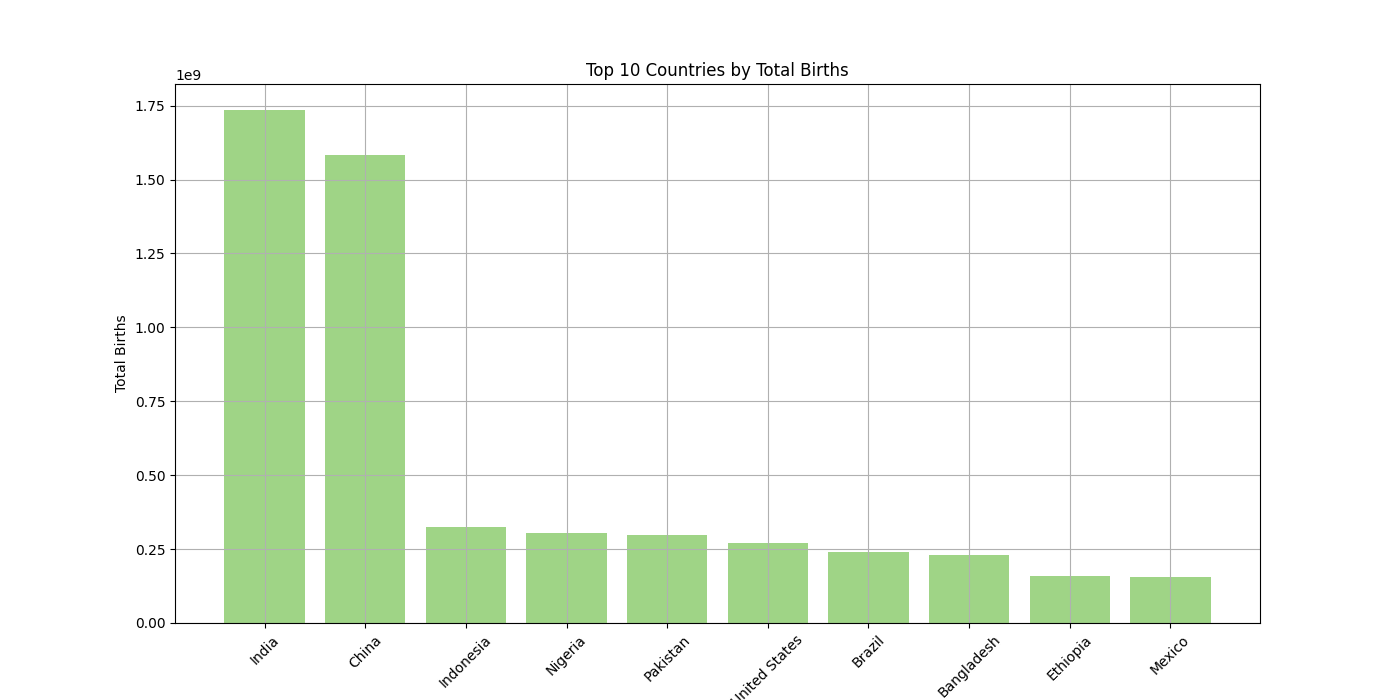
\includegraphics[width=0.5\textwidth]{img/前十个出生人数最多的国家的柱状图.png}
        \caption{前十个出生人数最多的国家的柱状图}
        \label{4}
    \end{figure}

    \begin{figure}[h!]
        \centering
        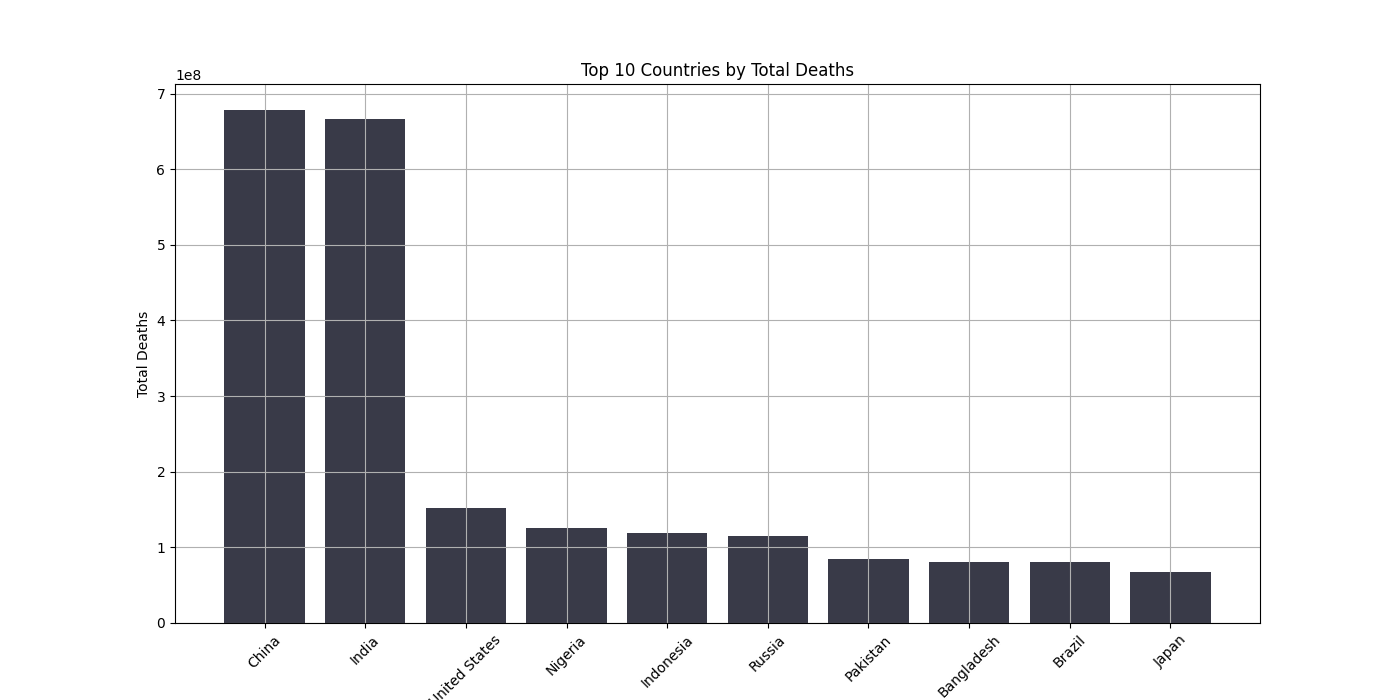
\includegraphics[width=0.5\textwidth]{img/前十个死亡人数最多的国家的柱状图.png}
        \caption{前十个死亡人数最多的国家的柱状图}
        \label{5}
    \end{figure}

    \begin{figure}[h!]
        \centering
        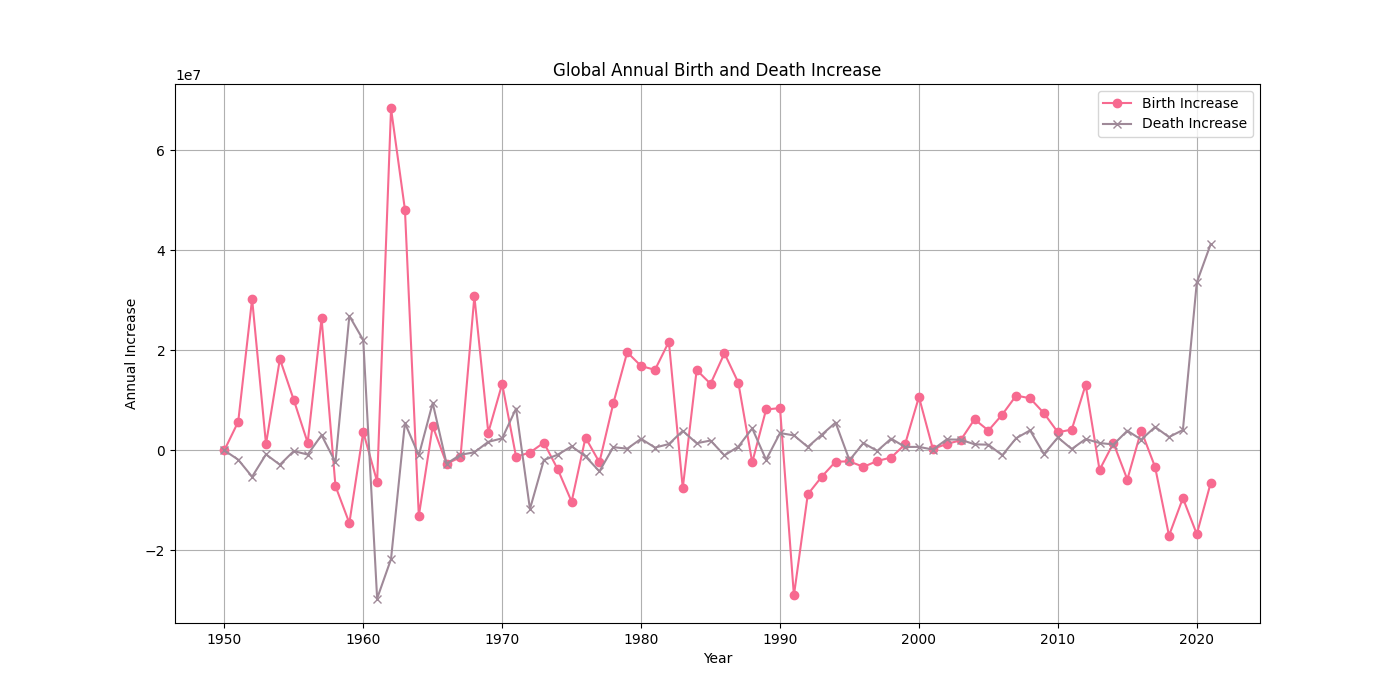
\includegraphics[width=0.5\textwidth]{img/全球每年新增出生和死亡人数的折线图.png}
        \caption{全球每年新增出生和死亡人数的折线图}
        \label{6}
    \end{figure}

    \begin{figure}[h!]
        \centering
        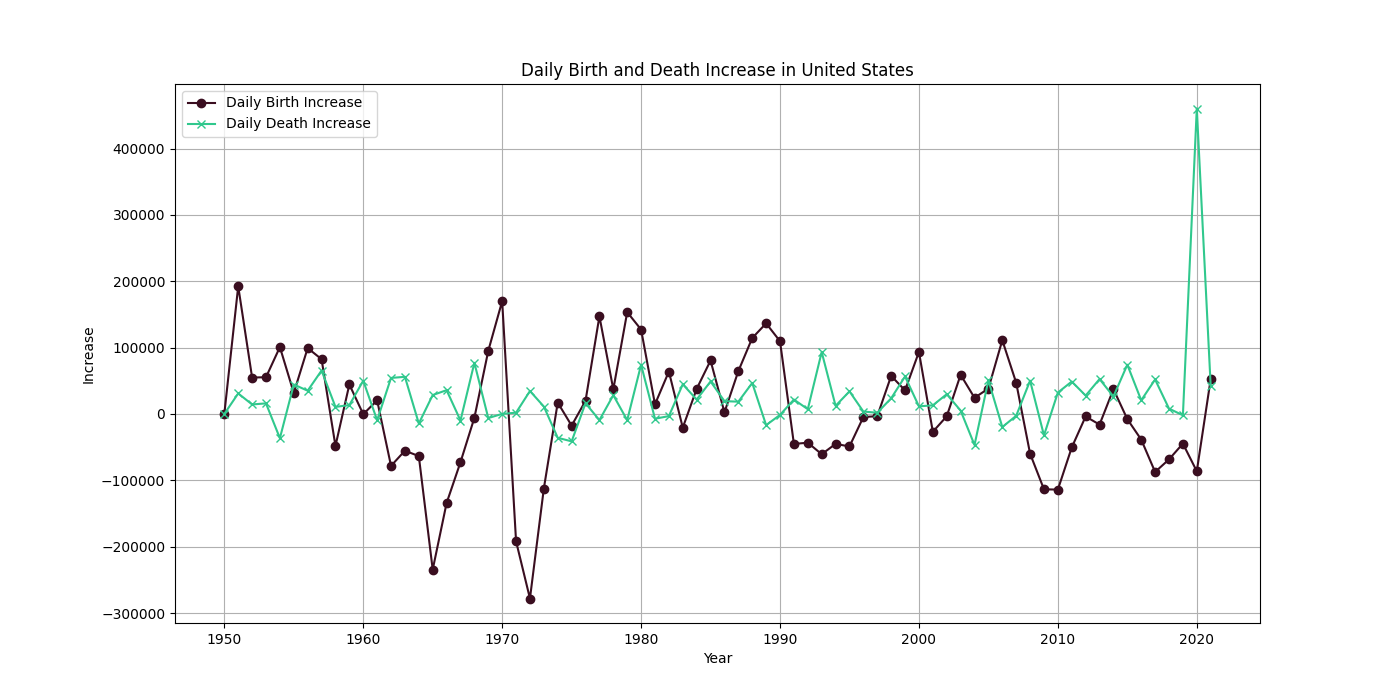
\includegraphics[width=0.5\textwidth]{img/United States出生死亡人数折线图.png}
        \caption{United States出生死亡人数折线图}
        \label{7}
    \end{figure}

    \begin{figure}[h!]
        \centering
        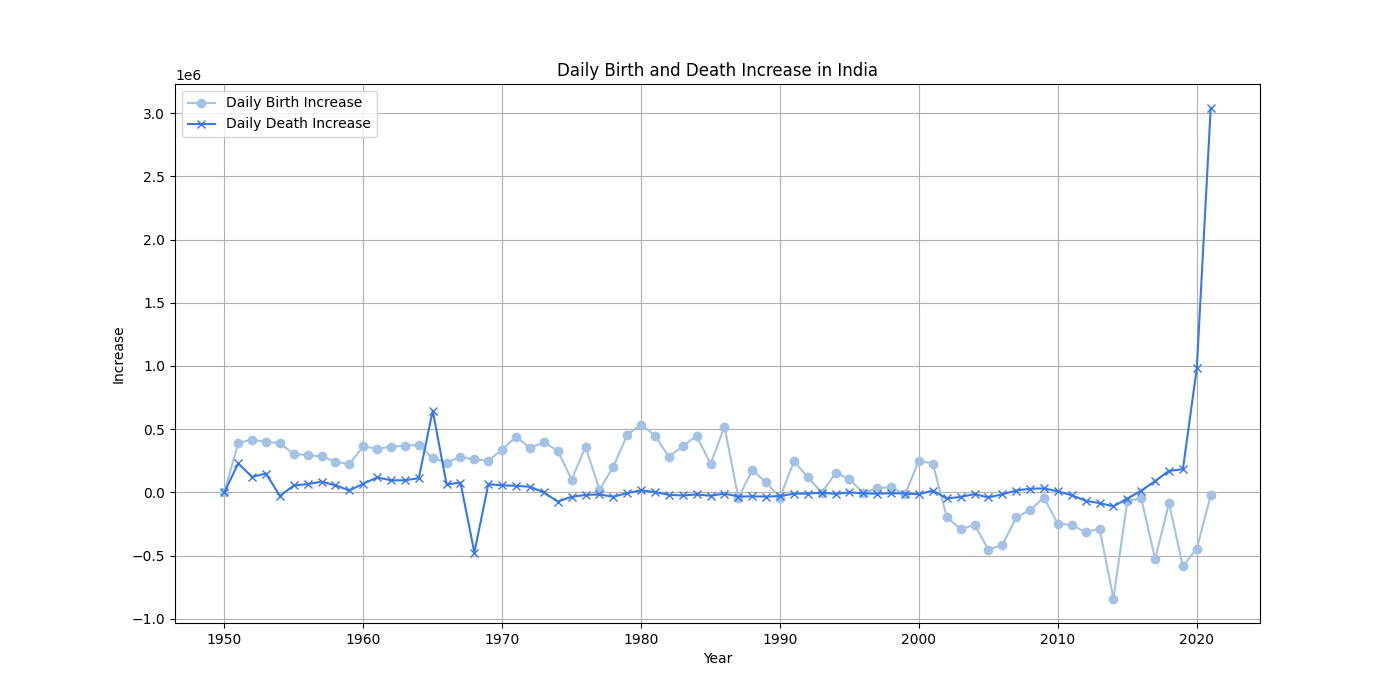
\includegraphics[width=0.5\textwidth]{img/India出生死亡人数折线图.png}
        \caption{India出生死亡人数折线图}
        \label{8}
    \end{figure}

    \begin{figure}[h!]
        \centering
        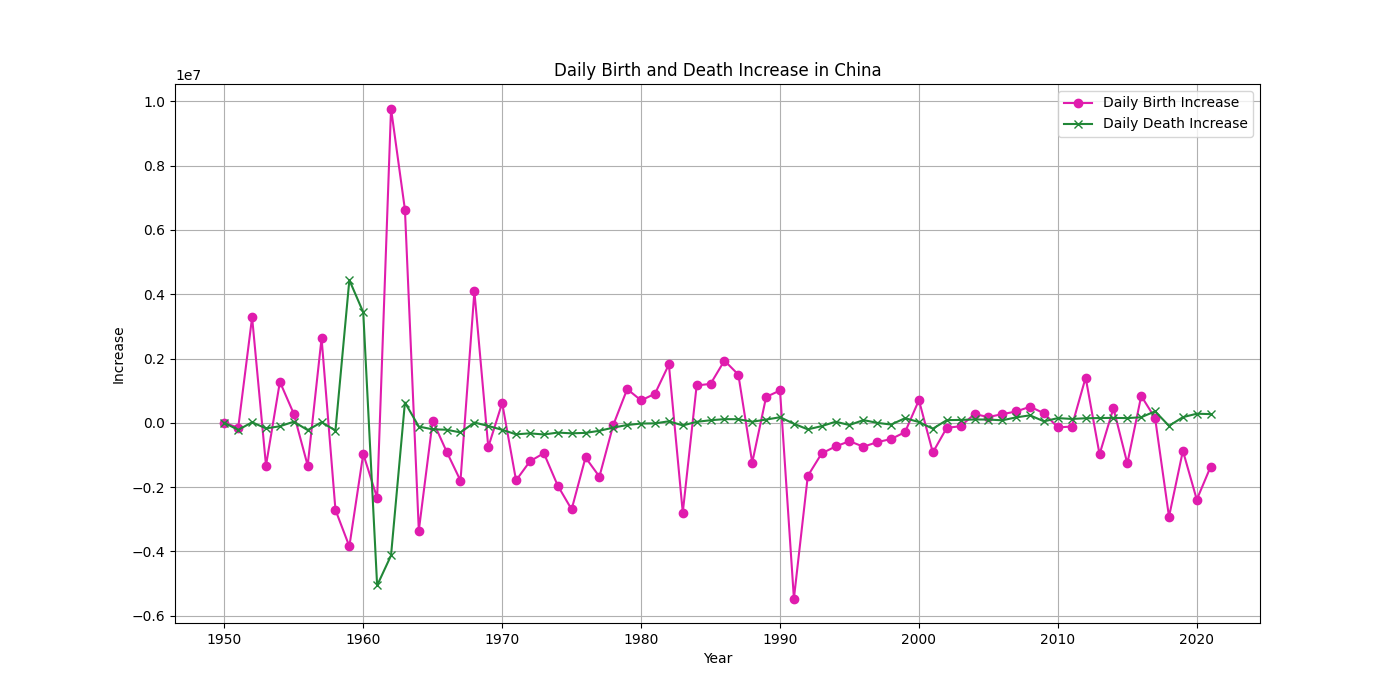
\includegraphics[width=0.5\textwidth]{img/China出生死亡人数折线图.png}
        \caption{China出生死亡人数折线图}
        \label{9}
    \end{figure}

    \begin{figure}[h!]
        \centering
        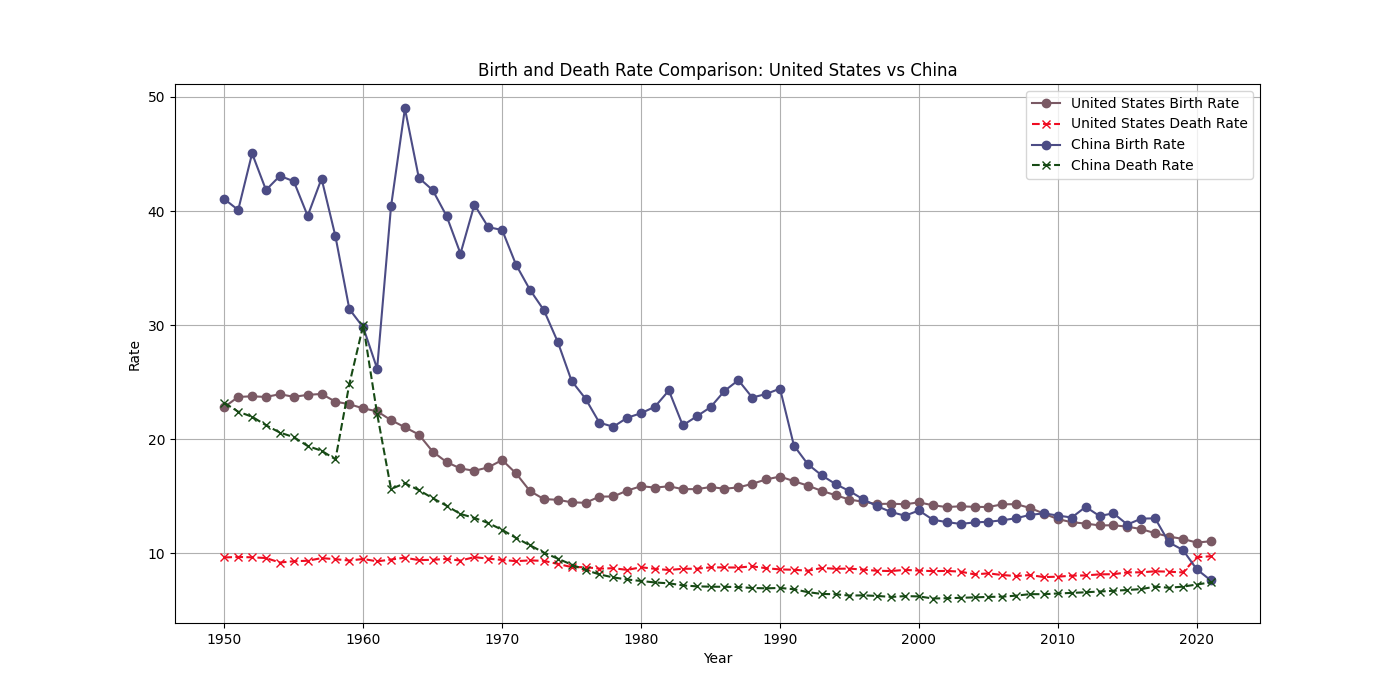
\includegraphics[width=0.5\textwidth]{img/United States_China比较.png}
        \caption{United States和China比较}
        \label{10}
    \end{figure}

    
    %\newpage
    %\bibliographystyle{alpha}
	%\bibliography{refs}
    %参考文献,写在refs.bib

    
\end{document}
